% !TEX encoding = UTF-8 Unicode
%!TEX TS-program = xelatex

\documentclass[12pt]{extarticle}
% extarticle is like article but can handle 8pt, 9pt, 10pt, 11pt, 12pt, 14pt, 17pt, and 20pt text

\def \ititle {Origins of Mind}
 
\def \isubtitle {Lecture 08}
 
\def \iauthor {Stephen A. Butterfill}
\def \iemail{s.butterfill@warwick.ac.uk}
\date{}

%for strikethrough
\usepackage[normalem]{ulem}

\usepackage{pdfpages}


\input{$HOME/Documents/submissions/preamble_steve_handout}

%logic symbol \leftmodels
\usepackage{MnSymbol}

%\bibpunct{}{}{,}{s}{}{,}  %use superscript TICS style bib
%remove hanging indent for TICS style bib
%TODO doesnt work
\setlength{\bibhang}{0em}
%\setlength{\bibsep}{0.5em}


%itemize bullet should be dash
\renewcommand{\labelitemi}{$-$}

\begin{document}

%\raggedcolumns

\begin{multicols*}{3}

\setlength\footnotesep{1em}


\bibliographystyle{newapa} %apalike

%\maketitle
%\tableofcontents




%--------------- 
%--- start paste
\def \ititle {Logic I}
 
\def \isubtitle {Lecture 16}
 
\begin{center}
 
{\Large
 
\textbf{\ititle}: \isubtitle
 
}
 
 
 
\iemail %
 
\end{center}
 
Readings refer to sections of the course textbook, \emph{Language, Proof and Logic}.
 
 
 
\section{There Is Exactly One}
 
There is one creator (at least one, maybe more).
 
\hspace{3mm} ∃x Creator(x)
 
Ahura Mazda is the one and only creator.
 
\hspace{3mm} Creator(a) ∧ ∀x( Creator(x) → x=a )
 
All squares are broken.
 
\hspace{3mm} ∀x( Sqr(x) → Brkn(x) )
 
There is one and only one creator.
 
\hspace{3mm} ∃y( Creator(y) ∧ ∀x( Creator(x) → x=y ) )
 
\hspace{3mm} or:
 
\hspace{3mm} ∃y ∀x( Creator(x) ↔ x=y )
 
 
 
\section{Every Time I Go to the Dentist Someone Dies}
 
\emph{Reading:} §11.2
 
∀t (
 
\hspace{5mm} ( Time(t) ∧ ToDentist(a,t) )
 
\hspace{5mm} →
 
\hspace{5mm} ∃x ( Person(x) ∧ TimeOfDeath(x,t) )
 
)
 
 
 
\section{Could There Be Nothing?}
 
\emph{Reading:} §13.2
 
\begin{center}
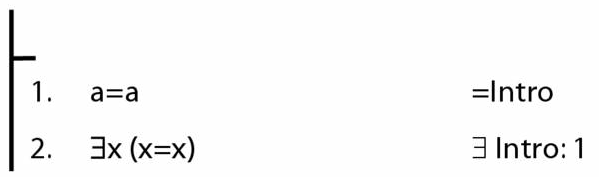
\includegraphics[scale=0.3]{img/uni_805_proof1.png}
\end{center}
\begin{center}
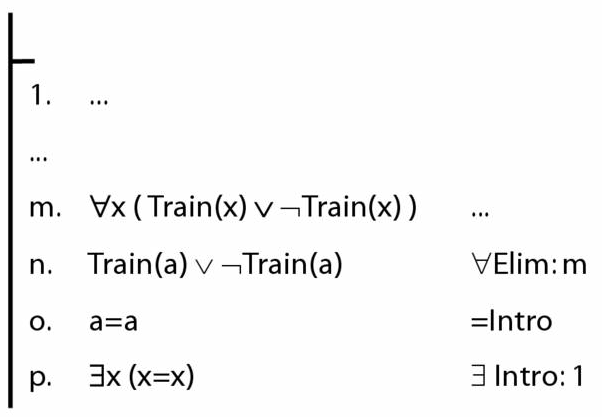
\includegraphics[scale=0.3]{img/uni_805_proof2.png}
\end{center}
\begin{center}
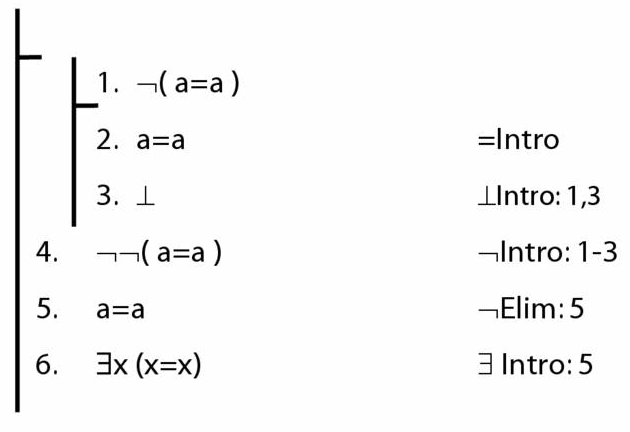
\includegraphics[scale=0.3]{img/uni_805_proof3.png}
\end{center}
 
 
\section{Proofs about Proofs}
 
\begin{minipage}{\columnwidth}
 
\textbf{If A $\vdash$ B then $\vdash$ A→B}
 
Proof Given a proof for A $\vdash$ B …
 
\begin{center}
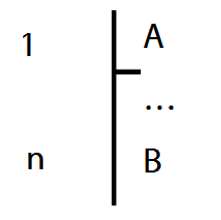
\includegraphics[scale=0.3]{img/unit_440_a.png}
\end{center}
… we can turn it into a proof for $\vdash$ A→B:
 
\begin{center}
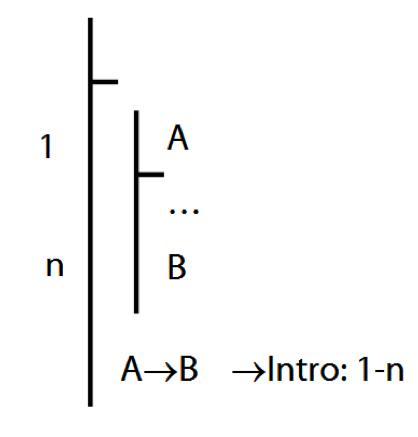
\includegraphics[scale=0.3]{img/unit_440_b.png}
\end{center}
\end{minipage}

\vfill 
 
\begin{minipage}{\columnwidth}
 
\textbf{If A $\vdash$ B then A $\vdash$ ¬¬B}
 
Proof:
 
\begin{center}
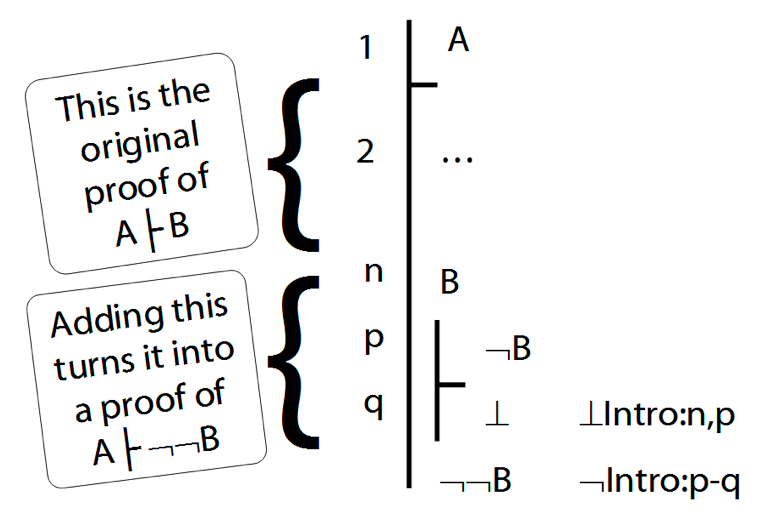
\includegraphics[scale=0.3]{img/unit_440_c.png}
\end{center}
\end{minipage}
 
\textbf{If A $\vdash$ C then A $\vdash$ B→C}
 
\textbf{If A $\vdash$ B and A $\vdash$ ¬C then A $\vdash$ ¬(B→C)}
 
 
 
\section{Does ‘if’ mean what ‘→’ means?}
 
\emph{Reading:} §7.3
 
\begin{minipage}{\columnwidth}
 
These two arguments are valid: does that mean that `if' means what `→' means?
 
\begin{center}
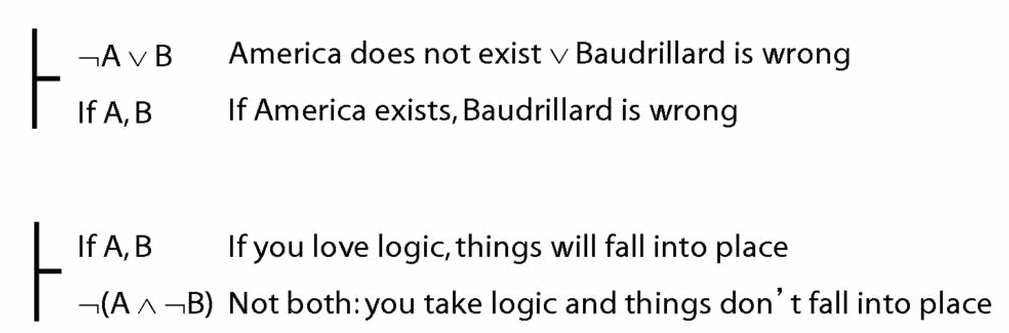
\includegraphics[scale=0.3]{img/if_is_arrow.png}
\end{center}
\end{minipage}
 
\begin{minipage}{\columnwidth}
 
The English argument isn't valid; the awFOL argument is valid; therefore `if' can't mean what `→' means?
 
\begin{center}
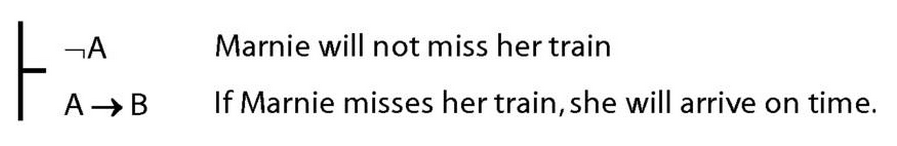
\includegraphics[scale=0.3]{img/if_aint_arrow.png}
\end{center}
\end{minipage}
 
%--- end paste
%--------------- 
 


\end{multicols*}

\end{document}